\section{Experiments}

In this section, we will first introduce the dataset and the compared methods. We will then further provide our models' results in the conventional depression detection setting and their efficacy and efficiency in ERD settings. We finally illustrate the explainability of the proposed method with examples.

\subsection{Dataset}

We mainly use the \textbf{eRisk2017} dataset \cite{losada2016test} in our experiment, which is adopted as the benchmark in the ERD task of CLEF 2017 \cite{losada2017erisk}. It consists of 137 depressed users and 755 control users and is divided into training/test set with 486/406 users each. The depressed users are identified with patterns like ``I was diagnosed with depression'', while the control users are those active on depression subreddit but had no depression. The posting year spans from 2007 to 2015. The anchor post for identification is filtered from the dataset. This filtering strategy can prevent the direct information leakage from the self-report, which may prevent the model from learning other indirect depression signals. We also conducted experiments and validated the generalizability of the proposed method on other two datasets with in-domain and cross-domain experiments (see Appendix). 

\subsection{Competing Methods}
We compare our method with several competitive baselines. For traditional machine learning models. \textbf{LR} uses TF-IDF features and a logistic regression classifier. \textbf{Feature-Rich} utilizes some additional user-based features, including LDA topic distribution \cite{blei2003latent}, LIWC features \cite{pennebaker2001linguistic} and emoticon counts. This is a competitive baseline that has been widely accepted in depression detection works on Facebook, Twitter and Reddit datasets \cite{eichstaedt2018facebook,trotzek2018utilizing,harrigian2020models}.

For neural baselines, we consider both models with large pretrained LM and relatively small models. For small models, we choose the representative \textbf{HAN-GRU} model \cite{zogan2021explainable}, which adopts a similar HAN structure with GRU as both the user encoder and post encoder. To have a fair competition with large models, it uses the last 1000 posts for classification, which is already a major portion of or the full posting list for many users. For large models, due to their computational cost and length limit, post selection is necessary. Therefore, each method is denoted as a pair of model and selection strategy. For backbone model, we consider the strong pre-trained model \textbf{BERT} and the proposed \textbf{HAN-BERT}. For post selection strategy, \textbf{Heuristic} chooses last posts in user history. \textbf{Clus} and \textbf{Clus+Abs} are inspired by \cite{zogan2021depressionnet}. We use sentence-bert \cite{reimers-2019-sentence-bert} to get post embeddings and run K-means clustering to get the $K$ posts nearest to the cluster center as representative posts (Clus). These posts are further passed to a BART model \cite{lewis2020bart} pretrained on CNN/DM summarization dataset to get an abstractive summary (Clus+Abs). Finally, the proposed screening strategy is denoted as \textbf{Psych}. 

The basis of BERT and HAN-BERT models are \texttt{bert-base-uncased}. The sentence-bert model is \texttt{paraphrase-MiniLM-L6-v2}. The number of selected posts is $K=16$. We train with a batch size of 4, and learning rate of 2e-5. We concatenate the selected posts as input into the BERT baselines. For HAN-BERT models, the user encoder is a 4-layer 8-head transformer encoder. To avoid the influence of randomness, we run each method with 3 different seeds and report the best performance.


\subsection{Conventional Setting Results}
\label{sec:conventional}

We first conduct experiments in conventional depression detection setting (Table \ref{table:erisk2017}). We can see that BERT (Clus+Abs) performs worse than BERT (Clus), indicating that the abstractive summarization strategy does not necessarily work possibly due to the gap between its pretrained domain (News) and Reddit. HAN-BERT (Clus) outperforms BERT (Clus), showing the effectiveness of the proposed HAN structure. The poor performance of HAN-BERT (Heuristic) highlights the importance of post selection, and none of the traditional post selection methods can outperform the competitive Feature-Rich model with access to all posts. However, with our proposed screening strategy, the HAN-BERT (Psych) model significantly outperforms baselines. HAN-GRU performs worse than HAN-BERT (Psych), suggesting the importance of a strong backbone model.

\begin{table}[t]
    \centering
    \small
    \begin{tabular}{l|c}
        \hline
        {} & F1 \\
        \hline
        LR & 60.2 \\
        Feature-Rich & 63 \\
        \hline
        HAN-GRU & 61.7 \\
        BERT (Clus) & 59.6 \\
        BERT (Clus+Abs) & 52.3 \\
        HAN-BERT (Heuristic) & 43.2 \\
        HAN-BERT (Clus) & 62.5 \\
        \hline
        HAN-BERT (Psych) & \textbf{70.3} \\
        % - Attention & 67.9 \\
        \hline
    \end{tabular}
    \caption{\label{table:erisk2017} Results on eRisk2017 test set.}
\end{table}

\subsection{Early Detection}

We then test model performance in the ERD setting, using the official metrics ERDE$_{5}$ and ERDE$_{50}$ \cite{losada2017erisk}. We also report F1 calculated using the early predictions (report positive if predicted probability over the predefined threshold 0.5, with which all these models are trained). We exclude baselines with unsatisfying performance and preserves LR, Feature-Rich and HAN-GRU. To tackle the item-by-item updates, the baseline models have to recalculate the features and run inference for each new post, while our HAN-BERT with risky post screening can deal this efficiently with the proposed evolving queue algorithm (\S \ref{sec:evolving}). When counting the running time, we accumulate the time costs for all posts no matter if the model makes early predictions to rule out the influence of early false positives. LR and Feature-Rich run on a Linux machine with CPU: E5-2678 (48 cores), while HAN-GRU and HAN-BERT run with a NVIDIA 2080 Ti GPU. Although the comparison is not totally fair, we think it is still a practical setting for real world applications.

\begin{table}[h]
    \centering
	\small
    \begin{tabular}{l|cccccc}
        \hline
        Model & ERDE$_5$ & ERDE$_{50}$ & F1 & Time(s) \\
        \hline
        LR & 13.70 & 8.49 & 40.5 & 4710.7 \\
        Feature-Rich & 12.98 & 8.39 & 35.8 & 7558.4 \\
        HAN-GRU & 13.30 & 8.58 & 40.7 & 19671.4 \\
        HAN-BERT (Psych) & \textbf{10.72} & \textbf{8.12} & \textbf{60.3} & \textbf{1330.3} \\
        \hline
    \end{tabular}
    \caption{\label{table:early} Test results on eRisk2017 in early detection setting. The lower ERDE$_5$ and ERDE$_{50}$, the better model performs early detection.}
\end{table}

The results are shown in Table \ref{table:early}. It can be seen that HAN-BERT (Psych) significantly outperforms baselines in ERDE and F1, while also being faster. The reason for the superiority on effectiveness is because baselines produce much more false positives than HAN-BERT due to their sensitivity to single posts. The advantage of efficiency can be mainly attributed to the evolving queue algorithm, which greatly reduced the number of model inference to only 10.41\% of all posts. The efficient feature update also helps. Although the sentence encoding must be conducted for all posts, it only costs a small fraction of total time (114.7s out of 1330.3s). The extremely long running time of HAN-GRU further highlights the importance of the proposed algorithm, as we can expect an unaffordable time cost for the even larger BERT-based models without it. 

\begin{figure}[h]
    \centering
    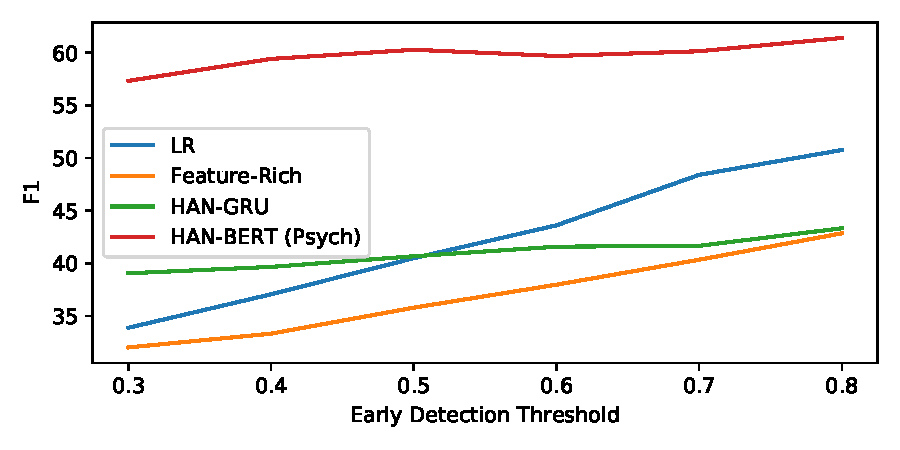
\includegraphics[width=0.88\columnwidth]{figures/thr2early_f1.pdf}
    \caption{Effect of threshold on early detection F1.}
    \label{fig:thr2early_f1}
\end{figure}

\begin{table*}[t]
    \centering
	\small
    \begin{tabular}{ccc}
        \hline
        Attention & Post & Diagnostic Basis \\
        \hline
        0.202 & \makecell[l]{It sucks that the Citalopram didn't work for you but glad to hear your other \\ meds are helping. It's my first time on antidepressants so I didn't know \\ what are their side effects.} & \makecell[c]{\textbf{Treatment} \\ Diagnosis \\ Changes in Appetite }\\
        \hline
        0.118 & \makecell[l]{Thanks! :) Sometimes it's really good to actually get the words out of  \\ me rather than internalising my feelings.} & \makecell[c]{Concentration Difficulty \\ Loss of Pleasure \\ \textbf{Self-Dislike}}\\
        \hline
        0.048 & \makecell[l]{Glad to know :) just glad I'm not working for the next couple of weeks. \\ Feel like I'm on a different planet haha.} & \makecell[c]{\textbf{Tiredness} \\ Stay still \\ Concentrate} \\
        \hline
        0.021 & \makecell[l]{Some films or TV shows. I remember watching ... The worst part was I'd  \\ already been laughed at by my mum for crying at the end of Breakfast at \\ Tiffanys (who leaves a cat out in the rain like that?). } & \makecell[c]{Sadness \\ \textbf{Crying} \\ Depressed Mood} \\
        \hline
        \end{tabular}
        \caption{\label{table:example} Example posting list (4 selected out of all 16 posts) of a user with depression with their attention weight in HAN and diagnostic basis according to top 3 cosine similarity (reasonable ones highlighted in bold).}
\end{table*}

We can adjust the detection latency $t$ by tuning the threshold and balance the tradeoff between precision and recall. Therefore, we hypothesize that model performance can be improved with varied threshold. We tune the threshold from 0.3 to 0.8, and check the changes in their early detection F1. This will run the risk of overfitting on the test set, but allow us to explore the best possible performance. As is shown in Figure \ref{fig:thr2early_f1}, the performance of baseline systems can improve by changing the threshold, but still fall behind HAN-BERT (Psych). Moreover, the performance of HAN-BERT (Psych) is not sensitive to threshold, so we may deploy it more comfortably without concerns on threshold tuning.

\subsection{Qualitative Example}

We provide a concrete example in Table \ref{table:example} to analyze the behaviors of HAN-BERT (Psych) in detail. From the column of attention weight, we can see that posts with strong depression indicators (e.g. antidepressants, internalizing feelings, see Row 1, 2) received much higher attention than a uniform baseline (1/16 = 0.0625), while posts with no evident signals of depression or even with a positive emotion (Row 3, 4) received low attention. This suggests the usefulness of the attention weight as an explanation for model prediction. The diagnostic bases decided by the cosine similarity between post and depression templates constitute another type of intuitive explanation. The top 3 diagnostic bases can usually capture the conventional depression behaviors that the post may indicate, which may act as a convincing interpretation in its clinical applications. However, we noticed that sometimes the similarity model may rank an unreasonable aspect high in the list of bases, such as the ``Sadness'' for the last positive post. We owe such mistakes to the limitation of sentence representation models, such as not sensitive to negation \cite{ribeiro2020beyond}. We expect stronger sentence representation models to alleviate the problem.
